\documentclass{article}
\usepackage[margin=0.5in]{geometry}
\usepackage[utf8]{inputenc}
\usepackage{hyperref}
\usepackage{color}
\usepackage{amsmath,amssymb}
\usepackage{mathtools}
\usepackage{mathrsfs}
\mathtoolsset{showonlyrefs}

\usepackage{minted}

\title{CMPSCI 390A Homework 3}
\author{\textbf{YOUR NAME HERE}}
\date{Assigned: Feb 11 2018; Due: Feb 18 2018 @ 11:00 am ET}

\begin{document}

\maketitle




\section{Comparing Linear Regression to $k$-NN}

\subsection{Performance Summary}

\begin{figure}[h]
    \centering
    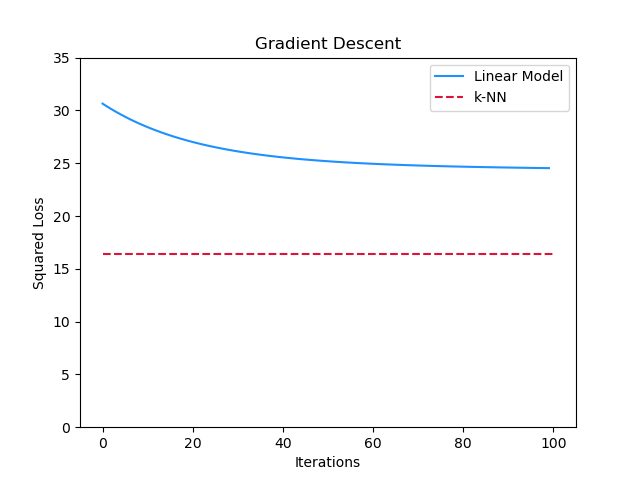
\includegraphics[width=0.5\textwidth]{images/learning_curve.png}
    \label{fig:learning_curve}
\end{figure}

\begin{table}[h]
\centering
\begin{tabular}{lllr}
\hline
\multicolumn{4}{c}{Regression Models}                                   \\ \hline
\multicolumn{1}{c}{Model} & \multicolumn{2}{c}{Hyperparameters} & Loss  \\ \hline
Linear Regression         & $\alpha = {value}$     & $N = {value}$    & {value} \\
$k$-NN                      & \multicolumn{2}{l}{$k = {value}$}       & {value} \\
\hline
\end{tabular}
\caption{Performances for each regression model.}
\label{tab:my-table}
\end{table}

\newpage
\subsection{Written Responses}

\begin{enumerate}
    \item (4 points) How did you optimize the hyperparameters for each method? Summarize your process in 3--5 sentences. \\
    
    \textcolor{blue}{your answer here}
    
    
    \item (4 points) Which method did you find easier to tune and why? (3--5 sentences) \\
    
    \textcolor{blue}{your answer here}
    
    \item (4 points) Propose a different loss function (other than least squares), and explain why it might be a reasonable alternative. (No more than approximately 250 words.)\\
    
    \textcolor{blue}{your answer here}
    
    \newpage
    \item (4 points) Consider that there are $n$ new data points, $(x_i, y_i), \dotsc$ and you are not allowed to refit $w$ to this new data. You are then asked to make predictions of the labels using the model $f_{w_N}$. In general, are these predictions likely to be better or worse than the predictions on the data used to find $w_N$? When do you think these predictions will be better and when would they be worse? (No more than approximately 250 words.)\\
    
    \textcolor{blue}{your answer here}
    
    \item (4 points) Propose a real-world problem, that we have not discussed in class, for which you might apply a regression algorithm. Describe the problem, what the features and labels correspond to, how much data we might have, and what loss function might be appropriate. Can you think of any practical concerns (or ethical issues) when it comes to actually using regression algorithms for this proposed problem? (No more than approximately 250 words.)
    \\
    
    \textcolor{blue}{your answer here}
    
\end{enumerate}

\newpage
\section{Extra Credit}

Your extra credit here. 

\end{document}
